\documentclass[11pt]{article}
	\title{Teoría de Autómatas y Lenguajes Formales\\[.4\baselineskip]Práctica 4: Numeración de Programas y EXWHILE}
    \author{Velasco Hurtado, Carlos}
    \date{\today}
    
    \addtolength{\topmargin}{-3cm}
    \addtolength{\textheight}{3cm}
	\usepackage{whilecode2}
	\usepackage{graphicx}
	\usepackage{amsmath}
	\usepackage{verbatim}

\begin{document}

\maketitle
\thispagestyle{empty}

\section{Exercise 1}
Create the simplest WHILE program that computes the diverge function (with zero arguments) and compute the codification of its code.
\\

\begin{whilecode}[H]

  $X1 \Assig X1 + 1$\;

 \While{$X1 \not = 0$}{
  $X1 \Assig X1$\
 }
 $X1 \Assig X1$

\end{whilecode}

Using the Octave script WHILE2N, the codification of this code is 9678230627.

\newpage

\section{Exercise 2}
Create an Octave script that enumerates all the vectors.
\verbatiminput{enumVectors.m}
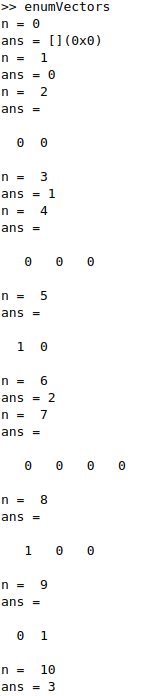
\includegraphics[scale=0.5]{enumVectors.png}
\newpage

\section{Exercise 3}
Create an Octave script that enumerates all the WHILE programs.
\verbatiminput{enumWhile.m}
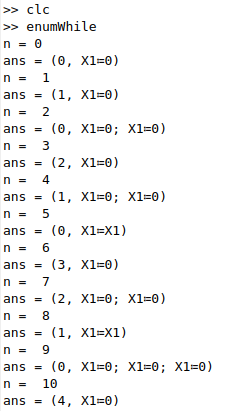
\includegraphics[scale=0.5]{enumWhile.png}

\end{document}

